\documentclass[11pt]{article}
\usepackage[top=1cm, bottom=2cm, left=1cm, right=1cm]{geometry}
\usepackage{ctex}
\usepackage{algorithm}
\usepackage{algorithmicx}
\usepackage{algpseudocode}
\usepackage{amsthm,amsmath,amssymb}
\usepackage[colorlinks=true,linkcolor=blue]{hyperref}
\usepackage{listings}
\usepackage{xcolor,xparse}
\usepackage{realboxes}
\usepackage{graphics}
\usepackage{graphicx}
\usepackage{mathrsfs}
\usepackage{wrapfig}
\usepackage{subfigure}
\usepackage{pifont}
\newcommand{\To}{\textbf{To} }
\definecolor{cmdbg}{rgb}{0.9,0.9,0.9}
\lstset{%
	basicstyle=\ttfamily,
	breaklines = true,
	backgroundcolor=\color{cmdbg},
}
\DeclareDocumentCommand{\ccmd}{v}{% 参数 v 表示工作方法类似于 \verb
    \Colorbox{cmdbg}{\csname lstinline\endcsname!#1!}%
}

\makeatletter
\newenvironment{breakablealgorithm}
  {% \begin{breakablealgorithm}
   \begin{center}
     \refstepcounter{algorithm}% New algorithm
     \hrule height.8pt depth0pt \kern2pt% \@fs@pre for \@fs@ruled
     \renewcommand{\caption}[2][\relax]{% Make a new \caption
       {\raggedright\textbf{\ALG@name~\thealgorithm} ##2\par}%
       \ifx\relax##1\relax % #1 is \relax
         \addcontentsline{loa}{algorithm}{\protect\numberline{\thealgorithm}##2}%
       \else % #1 is not \relax
         \addcontentsline{loa}{algorithm}{\protect\numberline{\thealgorithm}##1}%
       \fi
       \kern2pt\hrule\kern2pt
     }
  }{% \end{breakablealgorithm}
     \kern2pt\hrule\relax% \@fs@post for \@fs@ruled
   \end{center}
  }
\makeatother

\author{谢昀城 22307110070}
\title{计算物理作业6}

\begin{document}
\maketitle




  \section{题目1}
  \subsection{题目描述}
  
  Detecting periodicity: Download the file called sunspots.txt Download sunspots.txt, which contains the observed number of sunspots on the Sun for each month since January 1749. Write a program to calculate the Fourier transform of the sunspot data and then make a graph of the magnitude squared $|c_k|^2$ 
  of the Fourier coefficients as a function of 
  $k$—also called the power spectrum of the sunspot signal. You should see that there is a noticeable peak in the power spectrum at a nonzero value of 
 . Find the approximate value of $k$
  to which the peak corresponds. What is the period of the sine wave with this value of k?


\subsection{程序描述}
   在本程序中,我们通过对太阳黑子强度信号进行傅里叶变换求出其频谱,然后画出频谱的平方值随频率的变化图像。并给出频率峰值对应的周期,其中FFT由numpy库中的numpy.fft.fft函数实现。注意,由于信号均为正值,因此其FFT会有一个直流分量,我们在计算FFT后将其直流分量置零。

本程序源文件为FFTsunspots.py,在终端进入当前目录,使用命令python -u FFTsunspots.py运行本程序。运行时请保证Python第三方库Numpy,Matplotlib已安装。程序开发环境为Python3.12.3,可在Python3.8以上版本中运行。

\subsection{伪代码}
\subsubsection{计算周期 伪代码:}

\begin{breakablealgorithm}
  \begin{breakablealgorithm}
    \caption{Find Period}
    \begin{algorithmic}
        \State \textbf{INPUT:} $T$ (Time Series), $X$ (Number of the Sunspots)
        \State \textbf{OUTPUT:} $Tpeak$ (Period of FFT Peak)
        
        \State $X_{FFT} \gets FFT(X)$
        \State $Frequence \gets FFTFrequence(X,d={1\over 12})$
        \State $X|_{frequence=0}\gets 0$ \Comment{Remove DC Component}
        \State $fpeak \gets Frequence[ArgMax(Norm(X_FFT))]$
        \State \Return 1/fpeak
    \end{algorithmic}
    \end{breakablealgorithm}
    
  \end{breakablealgorithm}
  
  
  \subsection{输入输出实例}

  对于本程序,运行后会生成图\ref{fig:1}和图\ref{fig:2}为"FFT of sunspots.png"和"Original Signal and Dominant Component.png"于当前目录下,分别为信号的FFT结果和峰值附近的FFT结果,其中标注了峰值位置和原始信号图像和主要成分的图像。并会输出峰值的频率和周期。程序运行截图如图\ref{fig:3}所示。得到太阳黑子爆发的周期为10.91年

  \begin{figure}[ht]
    \centering
    \includegraphics[width=0.8\linewidth]{photo/FFT of sunspots.png}
    \caption{(a)sunspots 的频谱图(b)峰值附近的频谱图}
    \label{fig:1}
  \end{figure}

  \begin{figure}[ht]
    \centering
    \includegraphics[width=1.0\linewidth]{photo/Original Signal and Dominant Component.png}
    \caption{(a)sunspots信号的图像(b)sunspots主要频率成分的图像}
    \label{fig:2}
  \end{figure}

  \begin{figure}
    \centering
    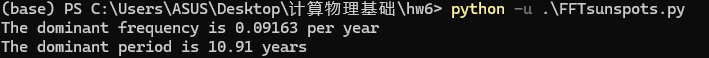
\includegraphics[width=0.6\linewidth]{photo/fig1.png}
    \caption{题目1程序运行截图}
    \label{fig:3}
  \end{figure}


\end{document}


